\lab{Python}{Optimization with Scipy}{scipy.optimize}
\label{lab:Optimization1}
\objective{Introduce some of the basic optimization functions available in \li{scipy.optimize}}

The Optimize package in Scipy has several types of optimizing algorithms.
This lab will introduce some of the basic types of algorithms included.

You can learn about all of the functions at \url{http://docs.scipy.org/doc/scipy/reference/optimize.html}.

First we will test out a few of the minimization algorithms on the Rosenbrock Function, which satisfies the equation $f(x,y) = (1-x)^2 + 100(y-x^2)^2$.
The Rosenbrock fuction is a common optimization algorithm checking function, so it is included in the optimize package, as well as its gradient (\li{rosen_der}) and its hessian (\li{rosen_hess}).

\begin{figure}
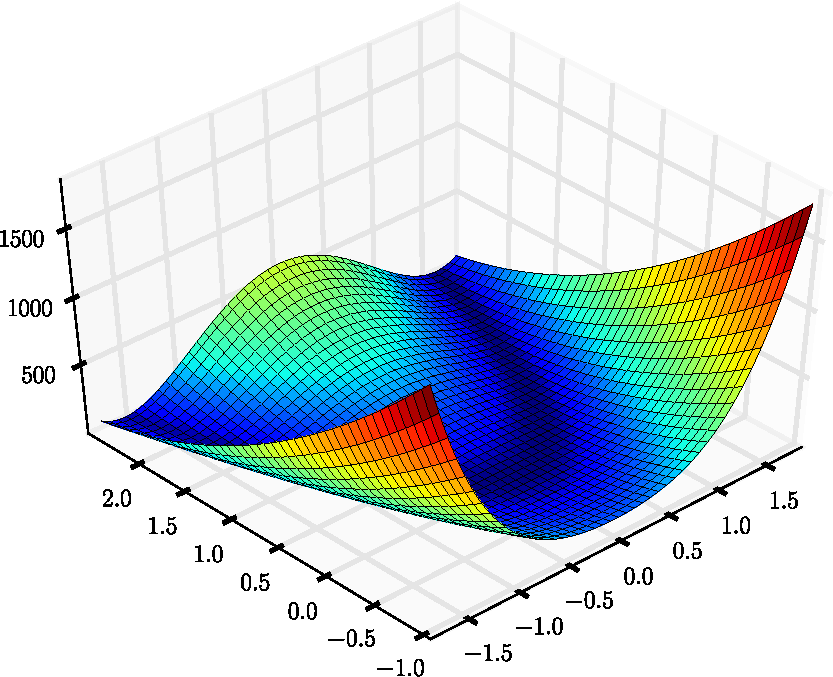
\includegraphics[width=\textwidth]{Rosenbrock.pdf}
\caption{$f(x,y) = (1-x)^2 + 100(y-x^2)^2$}
\label{opt:rosenbrock}
\end{figure}

We will use the \li{scipy.optimize.minimize} function and test each of its algorithms (under "method" on the online documentation page for \li{minimize}). Note that there are also several functions such as \li{fmin} and \li{fmin_powell}. These are equivalent to functions accsessed with the \li{minimize} function.

Note that for some algorithms, you'll need the jacobian (use \li{rosen_der}) and/or hessian.
You may recognize some of these algorithms, and several of them will be discussed in greater detail later. For this lab, you do not need to understand how they work.

\begin{problem}

Import the \li{scipy.optimize} module as \li{opt}. Now use the \li{opt.minimize} function to find the minimimum of the Rossenbrock function, found as \li{opt.rosen}. Test each of the algorithms. Part of the output of \li{opt.minimize} is the number of iterations each algorithm took. Which finds the minimum the fastest? Do any of the algorithms fail to find the (correct) minimum of the Rossenbrock?
Make sure to start with the same initial guess in all of them. As an example we'll minimize the Rossenbrock with the Nelder-Mead method.

\begin{lstlisting}
x0 = np.array([1.3, 0.7, 0.8, 1.9, 1.2])
opt.minimize(opt.rosen, x0, method='nelder-mead', options={'xtol': 1e-8, 'disp': True})
\end{lstlisting}

\emph{Extra: How would you maximize the Rossenbrock function?}
\end{problem}

When are optimizing functions, it is easiest when we are dealing with convex functions, as they only have one global minimum. However, this is frequently not the case, and sometimes we need pick the global minimum out of many local minima.

For example, consider the function
%This is the crazy function that I came up with to stump the algorithms
\[
z = r^2 (1+ 2sin(4r)^2)
\]
Where
\[
r = \sqrt{(x-4)^2 + y^2}
\]
Essentially this is a wavey crater offset from the origin by 1 along the $x$ axis.
\begin{figure}
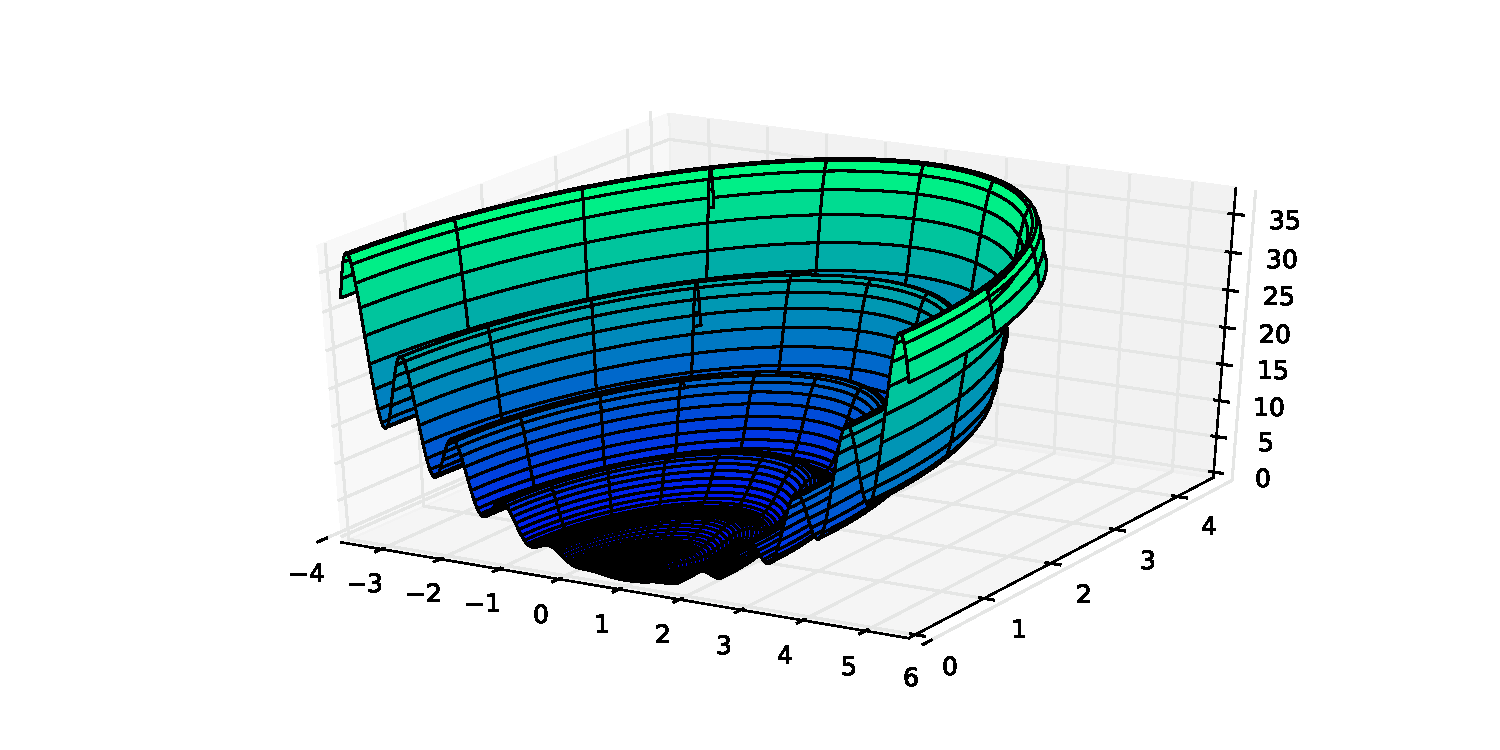
\includegraphics[width=\textwidth]{ManyMinima.pdf}
\caption{$z = r^2 (1+ 2sin(4r)^2)$}
\label{opt:muiltmin}
\end{figure}
This function has many local minima which we will see proves difficult for the minimization algorithms.

For example, if we use the \li{opt.fmin} function (which employs the Neader-Mead method, otherwise known as the downhill simplex method) the algorithm fails to find the global maximum, and instead comes to rest on a local maximum.
\begin{lstlisting}
def multimin(x):
    r = np.sqrt((x[0]+1)**2 + x[1]**2)
    return r**2 *(1+ np.sin(4*r)**2)

x0 = [-2,-2]
res = opt.fmin(multimin, x0, xtol=1e-8, disp=True)
print res
print multimin(res)
print multimin([-1,0])
\end{lstlisting}
Output
\begin{lstlisting}
Optimization terminated successfully.
         Current function value: 5.488169
         Iterations: 56
         Function evaluations: 134
[-2.03513929 -2.08611595]
5.48816865696
0.0
\end{lstlisting}

However, scipy does have some tools to help us with these problems. Specifically, we can use the \li{opt.basinhopping} function. 
Conceptually, most of the minimizing algorithms use to derivitive the function to search for the downhill direction of the function and make guesses downhill. Often they overshoot the minimum and come back. You can think of it as a ball rolling down a hill that slowly loses momentum as is overshoots the valleys and goes up the hill sides. Eventually the ball comes to rest at the bottom of a valley - hopefully the lowest valley. However, if there are many valleys (or loval minima) the ball can get stuck in one that's not the lowest valley.
The \li{opt.basinhopping} algorithim uses the same minimizing functions (in fact, you can tell it whatever minimizing algorithm you can pass to \li{opt.minimize}). However, once it settles on a minimum, the basinhopping algorithm pops it out of the this minimum (depending on how we set the "hopping" distance)  and hopefully out of the minimum its stuck it. If the new minimum it finds is even smaller than the last, it starts over with the new minimum.

\emph{Only Scipy Version 0.12+ has \li{opt.basinhopping}, in earlier versions, such as 0.11 you won't find it}
%I've seen a real cool animation of this -feasible to do in python?
\begin{problem}

Look at the documentation for the \li{opt.basinhopping} function online and use it to find the global minimum of our function with the same \li{x0}. Use the same \li{Nelder-Mead} algorithim with the same \li{xtol}. You will need to pass into the \li{opt.basinhopping} function a dictionary within a dictionary for the arguments of the minimizing algorithm to get all these options in.
Try it first with \li{stepsize=0.5} and then with \li{setsize=0.2}. Why doesn't it find the minimum the second time?

\end{problem}

The \li{optimization} package also has functions for root finding, for scalar functions and for multidimensional functions. The following example taken from the online documentation solves the following multidimensional system using \li{opt.root}.

\[
\begin{bmatrix}
	0 \\
	0
\end{bmatrix} = \begin{bmatrix}
	x_{0} + 1/2 ( x_{0} - x_{1} )^{3} - 1 \\
	1/2(x_{1}-x_{0})^{3} + x_{1}
\end{bmatrix}.
\]

\begin{lstlisting}
def func(x):
    return [x[0] + 0.5 * (x[0] - x[1])**3 -1.0,
            0.5 * ( x[1] - x[0])**3 + x[1]]
def jac(x):
    return np.array([[1 + 1.5 * (x[0] - x[1])**2,
                    -1.5 * (x[0] - x[1])**2],
                    [-1.5 * (x[1] - x[0])**2,
                    1 + 1.5 * (x[1] - x[0])**2]])
sol = opt.root(func, [0, 0], jac=jac, method='hybr')
print sol.x
print func(sol.x)
\end{lstlisting}

As with \li{opt.minimize}, \li{opt.root} has more than one algorithm for root finding. Here we use the \li{hybr} method, or the Powell hybrid method. There are also several algorithms for scalar root finding. See the online documentation for more.
%we still have curve fitting
%least squares programming -- but it seems that it's already been done in Volume One
Scipy also has functions to do curve fitting with the \li{opt.curve_fit} function. Just pass it data and a function to which to fit it to. The function should take in the independent variable as it's first argument and values for the fitting paramaters as subsequent arguments.
Examine the following example from the scipy.optimization online documentation.
\begin{lstlisting}
import numpy as np
import scipy.optimization as opt

#the function with which to create the data and later fit it
def func(x,a,b,c):
    return a*np.exp(-b*x) + c

#create the exact and random data
x = np.linspace(0,4,50)
y = func(x,2.5,1.3,0.5)
yn = y + 0.2*np.random.normal(size=len(x));

#perform the fit
popt, pcov = curve_fit(func,x,yn)
\end{lstlisting}
\li{popt} now contains the fitted parameters and \li{pcov} the covariance of the fit.
\begin{figure}
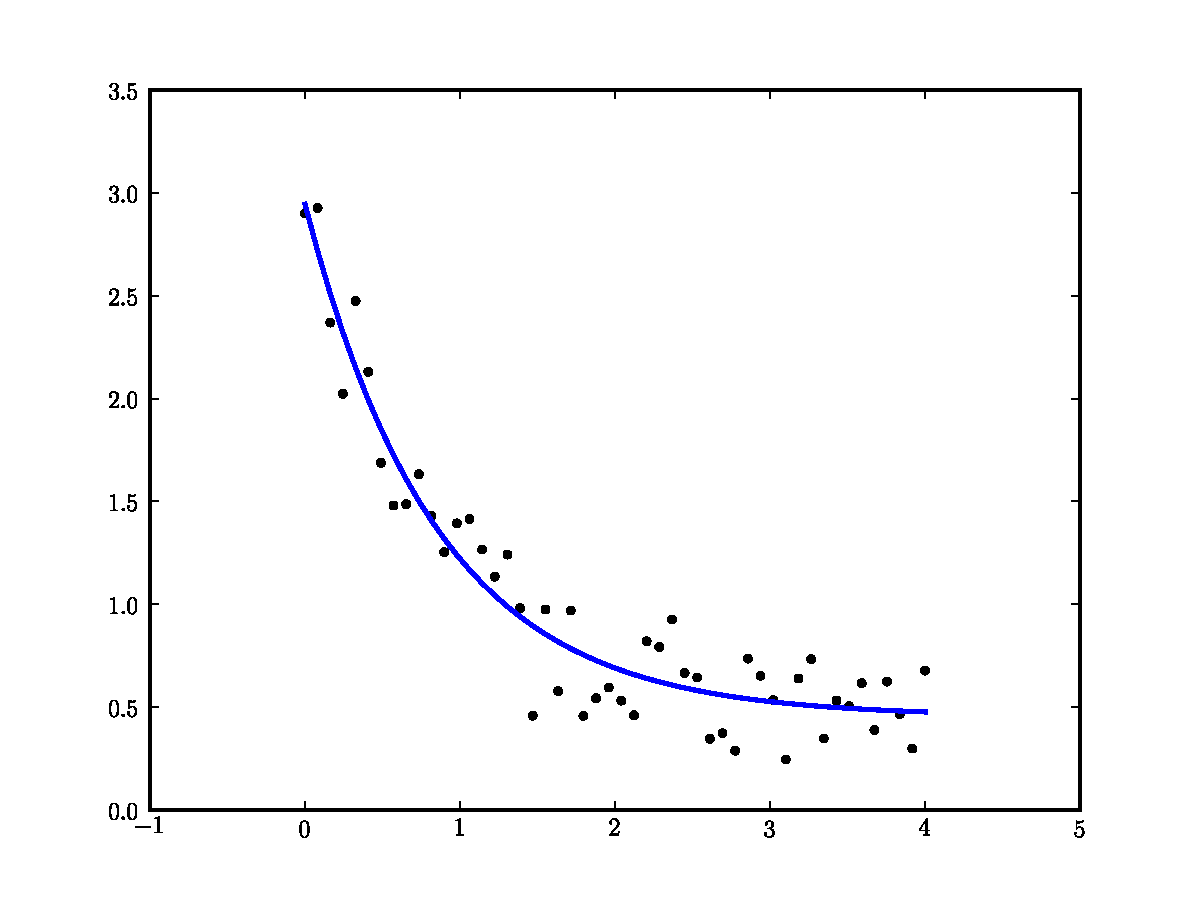
\includegraphics[width=\textwidth]{curve_fit.pdf}
\caption{Randomized data graphed with the curve using the fitted parameters:$a=2.72$,  $b=1.31$, and $c=0.45$ }
\label{opt:curve_fit}
\end{figure}
\begin{problem}
Use the \li{opt.curve_fit} function to fit a heating curve to data obtained from a temperature sensitive diode embeded in a cylindrical aluminum block. The temperature in the block was measured as it warmed from 290K up to 370K using a heating coil wound around the block attached to a copper rod which sat in a cooling bath of liquid nitrogen. 
Newton's law of cooling has the following form:
\[
T = T_{\infty} + \frac{P}{\gamma}+Ke^{\frac{\gamma t}{C}}
\]\
Where $T$ is the temperature, $t$ the time, $P$ the power used to warm it (which here was 59.43 watts), $T_{\infty}$ which was the ambiental temperature (290K), $\gamma$ a coefficient of heat tranfer through the copper rod, $C$ the total heat capacity of the block, and $K$ a constant coeffient the depends on the initial conditions. Use \li{opt.curve_fit} to find a fit to the data using $\gamma$, $C$, and $K$ as the fitting paramaters. Just so that you know that you are getting realistic values, $\gamma$ should be on the order of $10^{-1}$, $C$ on the order of $10^{2}$, and $K$ should be negative on the order of $10^{2}$.

From the heat capacity you obtained in the fit you can calculate the specific heat capacity of the aluminum block by dividing the heat capacity by the mass of the block (about 300g). Is it close to the expirementally measured specific heat capacity of aluminum of 0.900 J/g K? From $\gamma$ you can also calculate the thermal conductivity of the copper rod using the formula $k=\gamma L/A$ where $L$ and $A$ are the length ($25.6mm$) and the cross-sectional area ($71.24mm^{3}$) of the rod. How does it compare to the expirementally measured thermal conductivity of $401 W/(m \dot K)$? Look at the covariance you got from the fit. Is the error due to the fit, noise in the data, or an error in the expiremental setup?
\end{problem}

\begin{figure}
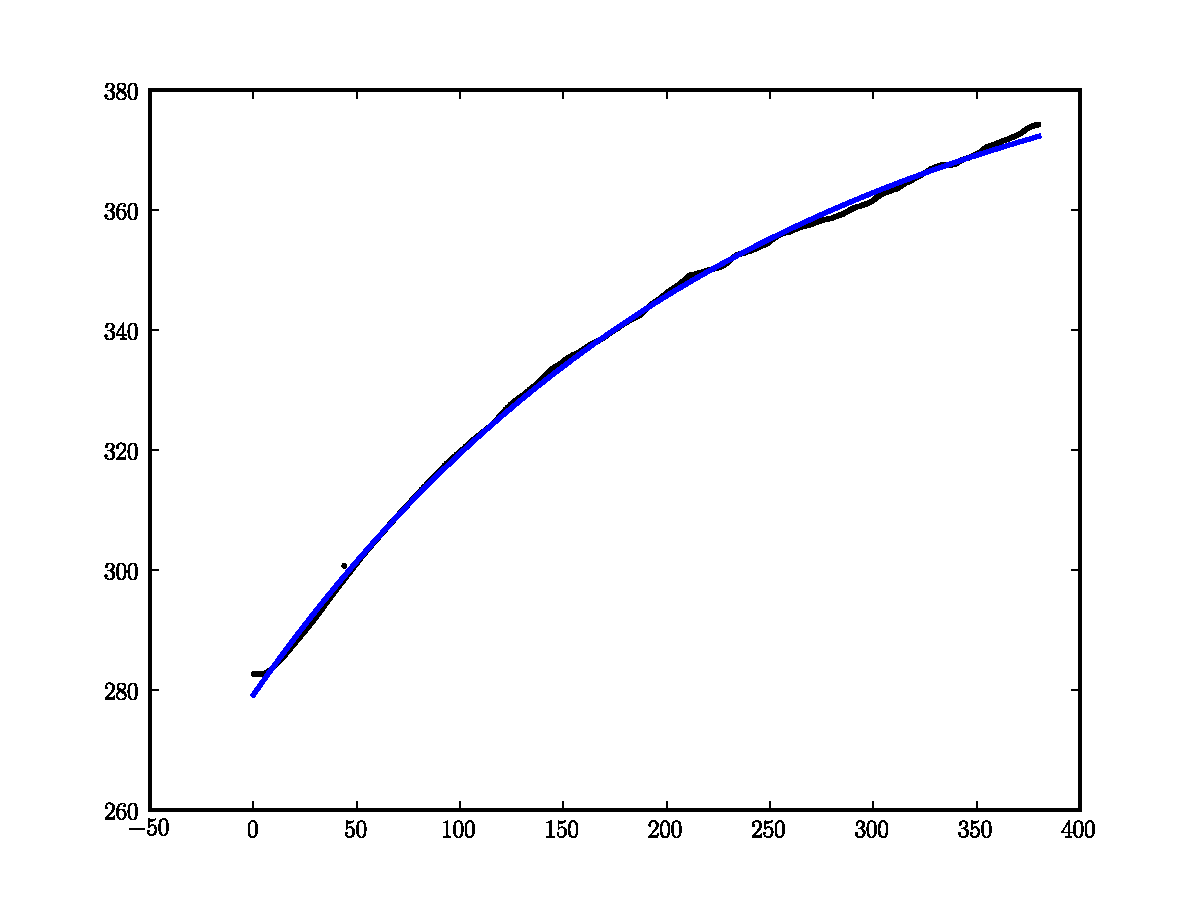
\includegraphics[width=\textwidth]{HeatingFit.pdf}
\caption{The black line is actually the data from \li{heating.txt} plotted as a scatter plot. It appears as a line because the data is very dense. The blue line is a fitted line. }
\label{opt:HeatingFit}

The \li{optimization} package also has many other useful functions, several 


